\documentclass{article} \usepackage{CJK}
\usepackage{CJK}
\usepackage{ctex}
\usepackage{graphicx}
\renewcommand{\contentsname}{目录}
\renewcommand{\abstractname}{摘要}
\author{杨铭 - 5130379022}
\title{《刺客信条:枭雄》分析测评}
\begin{document}
\maketitle
\tableofcontents
\newpage
\begin{abstract}
刺客信条是育碧公司十分出色的一系列游戏作品。自2007年发售第一款作品以来,每一款作品都收到了颇高的评价。但是一个系列,一个游戏模式做多了以后,总难免会让玩家审美疲劳。作为刺客信条发行时间线上第六部作品,《刺客信条:枭雄》(以下简称《枭雄》)不仅克服了前作《刺客信条:大革命》被人所诟病的许多缺点,而且做出了许多创新,获得了令人满意的评价。下面我就详细分析《枭雄》的游戏设计和它成功的原因。
\end{abstract}
\section{游戏介绍}
\subsection{基本信息}
\begin{table}[!hb]
\centering
\begin{tabular}{lc|lc}
  \hline
  游戏名: & 刺客信条:枭雄 & 发行日期: & 2015年11月19日 ( PC )\\\hline
  英文名: & Assassin's Creed Syndicate & 玩家人数: & 单人/联网\\\hline
  游戏类型:& 动作、潜行、刺杀 & 游戏平台: & PC/PS4/XBOX\\\hline
  开发引擎:& Anvilnex & 开发/发行商:& 育碧\\
  \hline
\end{tabular}
\end{table}
\subsection{配置要求}
    \paragraph{最低配置}
    \begin{description}
      \item[系统] Windows 7, Windows8.1, Windows10
      \item[处理器] Intel Core i5 2400s @2.5 GHz or AMD FX 6350 @ 3.9 GHz
      \item[内存] 6GB
      \item[显卡] NVIDIA GeForce GTX 660 or AMD Radeon R9 270
      \item[图像驱动] DirectX June 2010 Redistributable
      \item[硬盘] 50 GB
    \end{description}
    \paragraph{推荐配置}
    \begin{description}
      \item[系统] Windows 7, Windows8.1, Windows10
      \item[处理器] Intel Core i7-3770 @ 3.5 GHz or AMD FX-8350 @ 4.0 GHz
      \item[内存] 8GB
      \item[显卡] NVIDIA GeForce GTX 760(4GB)or the newer GTX 970(4GB) or AMD Radeon R9 280X(3GB)
      \item[图像驱动] DirectX June 2010 Redistributable
      \item[硬盘] 50 GB
    \end{description}
\section{内容概括}
\subsection{背景简介}
    \paragraph{}刺客信条每一作都会有一个城市作为玩家主要活动的区域,《枭雄》将这一城市定为了1868年维多利亚时代的伦敦,也算得上刺客信条系列最接近现代的背景。工业革命的背景下,玩家扮演的刺客的敌人自然而然变成了城市里的工业巨头和大资本家。与前作不同的一点在于,在《枭雄》中,有一对姐弟作为玩家可控制的角色。在游戏中玩家随意切换自己要使用的角色。《枭雄》中的伦敦,也比之前系列最大的城市——《大革命》中的巴黎大出了30\%左右。游戏保留并发扬了高自由度的传统,玩家可以在硕大的日不落帝国首都飞檐走壁,拉帮结派,体会工业时代刺客的感觉。
    \paragraph{}在剧情方面,游戏还是延续了单线剧情的特点。但是为了完成主线,玩家不得不做各种支线任务来提升自己角色的武器和能力。剧情虽然也是老套的打倒杀父仇人,夺回伦敦之云,但是过程中的许多任务却设计用心:躲避警察销毁证据、击晕恶霸交给警察、解放童工......更可以接受狄更斯、贝尔等名人的委托,跟他们一起完成任务,历史代入感更强。
\subsection{人物介绍}
\paragraph{雅各布·弗莱}
\begin{figure}[!h]
  \centering
  % Requires \usepackage{graphicx}
  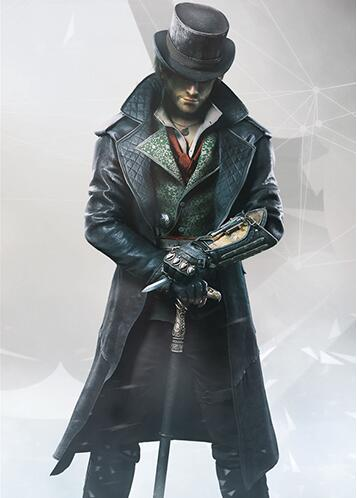
\includegraphics[width=15em]{jacob.jpg}\\
  \caption{Jacob}\label{1-1}
\end{figure}
\paragraph{}
雅各布·弗莱(Jacob Frye,1847 – 未知),出生于英国的克劳利,和他的姐姐自出生起便被当做刺客来抚养。在《枭雄》中来到伦敦,推翻圣殿骑士的统治,帮助贫苦群众。
\paragraph{}
作为游戏中的男主角,雅各布性格直率而且叛逆,喜欢黑帮老大的感觉,并且创建“黑鸦“组织跟圣殿骑士对抗。
\paragraph{伊薇·弗莱}
\begin{figure}[!h]
  \centering
  % Requires \usepackage{graphicx}
  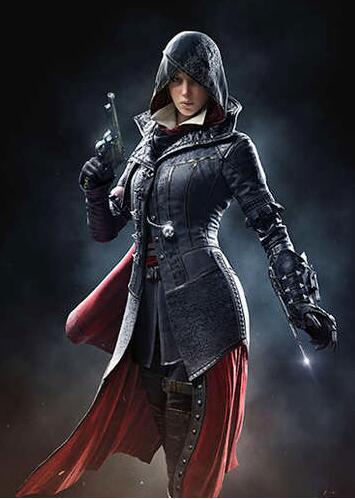
\includegraphics[width=15em]{evie.jpg}\\
  \caption{Evie}\label{1-2}
\end{figure}
\paragraph{}
伊薇·弗莱(Evie Frye,1847年 - 未知)是一名英国刺客,是雅各布的姐姐,比雅各布早4分钟出生。作为雅各布的姐姐,伊薇更加沉稳和冷静,她一直尽心尽力帮助弟弟的”黑鸦“与圣殿骑士斗争。
\paragraph{亨利·格林}
\begin{figure}[!h]
  \centering
  % Requires \usepackage{graphicx}
  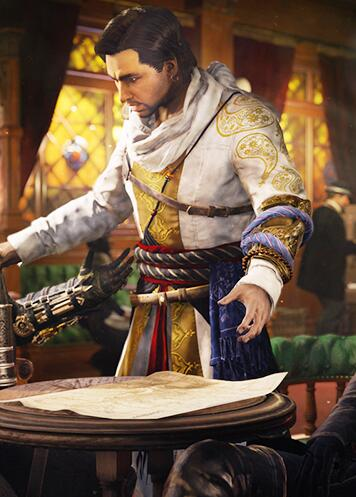
\includegraphics[width=15em]{henry.jpg}\\
  \caption{Henry}\label{1-3}
\end{figure}
\paragraph{}
亨利•格林(Henry Green),被称作幽灵(The Ghost),印度人,十九世纪60年代移民到英国,之后在伦敦成为了刺客的领导人,雅各布,伊薇•弗莱的好友。他是印度兄弟会刺客大师阿尔巴兹•米尔之子。
\paragraph{}
在游戏中,亨利作为玩家的向导出现,可以说是贯穿主线的“教程NPC”。
\subsection{游戏逻辑}
\paragraph{总述}
刺客的本质就是刺杀,为了完成刺杀的目标,潜行也是必须的。玩家需要扮演一个刺客,以各种方式杀掉自己的敌人——圣殿骑士,来夺回伦敦。\\
《枭雄》延续了前作的大部分玩法,也创新了一些新的操作和玩法:
\paragraph{传统}
\begin{description}
  \item[刺杀] 背后刺杀、双重刺杀、空中刺杀、双重空中刺杀......这些熟悉的动作让人屡试不爽
  \item[跑酷] 在高楼大厦见飞檐走壁,甚至借助船只、火车来完成跑酷动作。操作熟练的玩家会大呼过瘾
  \item[成长] 成长系统基本延续前作,包含装备和技能。而装备的升级功能从上作拖沓的五级制变为了两级制
  \item[敌人] 合理的敌人设定也提高了游戏乐趣:看到同伴尸体会警戒、头目见势不妙就逃走......
  \item[武器] 主武器、枪支、弩、烟雾弹、迷幻毒针,熟悉的武器,熟悉的操作,熟悉的味道。
  \item[藏身地] 藏身地也就是玩家的总部,可以在这里进行一些装备的更换和任务的交接。值得一提的是《枭雄》中的藏身地在一辆奔驰的火车上。
\end{description}
\paragraph{创新}
\begin{description}
  \item[马车] 第一次让我坐上马车,我是拒绝的,因为我觉得那是GTA。但是在比前作大30\%的地图上游戏,一个便捷的交通工具也是必须的。马车还可以作为作案工具,藏匿被打晕的圣殿骑士头目,甚至会有“车战”的发生。
  \item[滑索] 滑索可以让玩家在多座高楼间任意穿梭,更能完成前作不可能完成的空中刺杀动作。而且这个滑索还是大名鼎鼎的发明家贝尔制作的
  \item[切换角色] 可以自由切换弟弟和姐姐作为自己操控的人物,并且两人有各自擅长的刺杀技巧,灵活使用会让你事半功倍,当然代价就是由于两个角色不通用等级,你需要双份的游戏时间
  \item[帮派] 游戏将伦敦分为了几个区域,玩家需要在一个区域完成足够的任务,才能提升自己帮派在该区域的威信。同样高的帮派威信会让你在该区域内如鱼得水。另外帮派资源还能点亮一些辅助功能,帮你更好地完成任务。
\end{description}
\paragraph{}
总的来说,《枭雄》在主要游戏模式上没有太大的突破,游戏希望在“刺客”的路上精益求精,做出了许多努力让玩家能够更舒适地体验刺客的感觉。
\section{四要素分析}
\subsection{总述}
如何让玩家真正喜欢上自己的游戏,是许多游戏制作者朝思暮想的事情。育碧作为游戏行业的巨头,当然心里有谱。在至关重要的“游戏四要素”中,育碧根据《枭雄》的游戏类型、受众特点,为它量身打造了一款外衣,将剧情、美工、技术、机制
完美融入,相得益彰。
\subsection{剧情}
\paragraph{}
熟悉刺客信条系列的玩家都知道,每一部刺客信条都分为“现代”和“历史“两个剧情线。刺客信条的剧情是连贯的,设定也比较宏达和玄幻。故事设定在人类出现之前,地球上生活着一个叫”第一文明“的高等种族。他们创造了人类当做劳动力,并且用叫做”伊甸碎片“的
东西来控制人类。后来,第一文明被一场巨型太阳耀斑毁灭,但是第一文明在消失之前留下了许多生机,第一文明的三位伟人尝试了许多方法来挽救自己的族人,虽然没有成功,但其中一个叫做”朱诺“的第一文明伟人改变了其中一个方法”眼“的机制,让它一旦被启动
就会让朱诺的思维数字化覆盖整个地球。这听上去十分虚幻,从本质上来说就是地球会被朱诺所控制。而且第一文明也预测到第二次危机即将到来。
\paragraph{}
另一方面,游戏设定中用科学解释了“转生”的概念。我们的主角是历史上许多著名刺客的后代,在使用了一种仪器后,便可以进入他祖先的记忆中,从历史长河中找到第一文明的遗迹,挽救人类于毁灭之中。但是事情显然不会这么简单,“圣殿骑士”就是组织玩家的主力,
而且还有类似“朱诺”的化身,和“朱诺”的丈夫的转生这种神祗来误导主角。
\paragraph{}
虽然说了这么多,但是这都是刺客信条前几代的剧情。自从《刺客信条3》中戴斯蒙死后,《刺客信条》的剧情一直没有大的发展,《枭雄》也一样,剧情在向平淡化发展。宏达的世界观设定在前几部已经被玩家摸透以后,这种玄幻外加科幻的设定似乎也不能当做什么卖点,
《枭雄》的剧情不能给玩家什么惊喜,只能期望育碧能在后作中有所突破吧。
\subsection{美工}
\paragraph{}
作为一个真实画面3D游戏,《枭雄》跟它的《刺客》兄弟一样,力求打造一个贴合历史的高质量画面,这也是现在许多大游戏的基本要求。
\paragraph{}
根据作品定位的时代特征,整个游戏有些蒸汽朋克风格,比如进入游戏时的loading画面和许多游戏内场景的布置。在育碧更新了他们的游戏引擎Anvilnex后,游戏的画面也有不少的提升。但是《枭雄》并未向为人诟病的前作《大革命》一样在优化上栽跟头。这一作里,
玩家的主机即使没有很高的配置,依旧能够享受加高的游戏画面和稳定的帧数。当然,想要体验特效全开的快感,还是需要GTX980甚至更好的显卡才行了。
\paragraph{人物}
不仅是场景,人物的穿着和打扮也经过了育碧的精心打磨,玩家那标志性的刺客服饰也被渲染上了工业时代的颜色。圣殿骑士红色格子的标志性穿着也符合英国维多利亚时代乡绅的模样。
\begin{figure}[!h]
  \centering
  % Requires \usepackage{graphicx}
  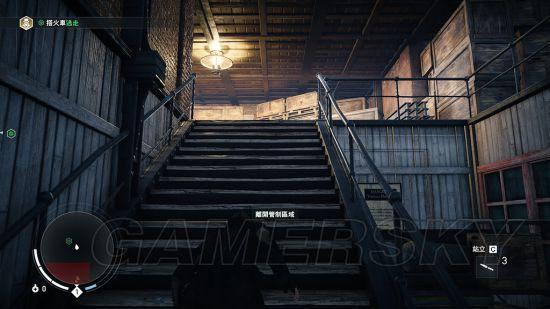
\includegraphics[width=20em]{scene1.jpg}\\
  \caption{逼真的光照}\label{2-1}
\end{figure}
\paragraph{}
总的来说,作为第一人称动作类(刺杀、潜行)游戏,《枭雄》的美工简直就是游戏的门面。而育碧并没有让玩家失望,游戏的每一个场景,每一个人物,乃至每一个道具和UI界面都和游戏背景完美融合,更升华了游戏的内涵。以至于许多场景去掉游戏UI的截图就可以当做
桌面壁纸。
\subsection{技术}
\paragraph{}
除去VR、AR等尚未普遍推广的技术,《枭雄》跟其他大多大游戏一样,追求的是高质量的画质,这也是大多数高端技术应用的地方。由于我没有获得《枭雄》开发的详细过程,只能以玩家的角度推断一些游戏所使用的技术。
\paragraph{头发}
头发的处理一直是真实性画面游戏的一个难题。真实的人类头发数量庞大,想要模拟出来并不容易。刺客信条采用了Nivida的HairWorks技术,开启以后,主角的头发将由五十万根独立的发丝渲染。这些发丝由特殊的运算技术配合GPU硬件整体一次完成运算。经过HairWorks
处理过的头发将会告别一块块“肉疙瘩”的形状,甚至可以适应各种环境变化,比如一阵风吹过,主角的头发将会随风飘扬,不禁让人想起“海飞丝”的广告词。
\paragraph{光影}
《枭雄》支持Nivida最新的PCSS技术,能够以较高的效率生成软阴影,使得游戏中的阴影有正常的模糊的边缘,看上去更加自然。
\paragraph{}
同时游戏也支持N卡的HBAO+环境光遮蔽技术,使得游戏在光影效果下呈现出震撼的画面。
\paragraph{}
\textbf{“我们不得不等待技术迎头赶上......现在的技术还不足以打造这样一个如此美丽的城市(伦敦)”}育碧魁北克的创意总监Marc-Alexis在采访中这样说道。
\paragraph{}
可以说,《刺客信条》的画面一直站在游戏界的前沿,这次更是下足了功夫,在优化上做足了功夫,才打造出了这样一个犹如历史画卷中的伦敦。
\subsection{机制}
\paragraph{}
游戏的机制在前面也有提及,《枭雄》没有脱离它的前作,基本延续了前作的机制。
\begin{description}
  \item[刺杀和割草] 虽然很多人把《刺客信条》归为刺杀或者潜行类,但是我更倾向于认为它仍是一款ARPG。游戏中的许多情况下玩家更像是一个战士,在进行“无双割草”而非刺杀。而刺激地砍杀和冷静地刺杀同样能给人带来游戏的快感。
  \item[主线和支线] 玩家在开放的区域内可以自由活动,但是你只有一条主线可以选择。单线剧情拯救了一些选择困难症和全剧情强迫症但也降低了剧情的自由度,但是有了高自由度的活动区域,单主线貌似也不是什么问题了,毕竟众多支线任务已经让人眼花缭乱了。
  \item[跑酷和潜行] 有时需要悄无声息,有时又需要迅捷如风,游戏给玩家设定了许多任务,让玩家可以体会跑酷或是潜行的快感。比如追逐任务、挟持任务、还有在高处自己等级许多的场景的暗杀。
\end{description}
\paragraph{}
说了那么多,其实《枭雄》的机制本质上就是虚拟的工业时代的伦敦。玩家可以在这个虚拟的伦敦里自由行动,只不过在你的地图上总有那么几个标志,提醒着你身为一个“刺客”的使命——“快去接任务啊!”。这种高自由度的游戏也是近些年许多游戏的惯用套路——
《看门狗》、《GTA5》......从这个角度来看,《枭雄》并没有什么突破,它只是延续了这个时代游戏的模式,我相信这也是未来游戏所努力的方向。
\section{结语}
\paragraph{}
《枭雄》作为刺客信条正统作品的第六代,于剧情和机制上没有什么突破,但是在机制上有些优化,在画面和技术上也是跟上时代的步伐。《枭雄》的发布也更加谨慎,避免了《大革命》被人称为“大BUG”的窘境,也获得了广大玩家的认可。
\begin{figure}[!h]
  \centering
  % Requires \usepackage{graphicx}
  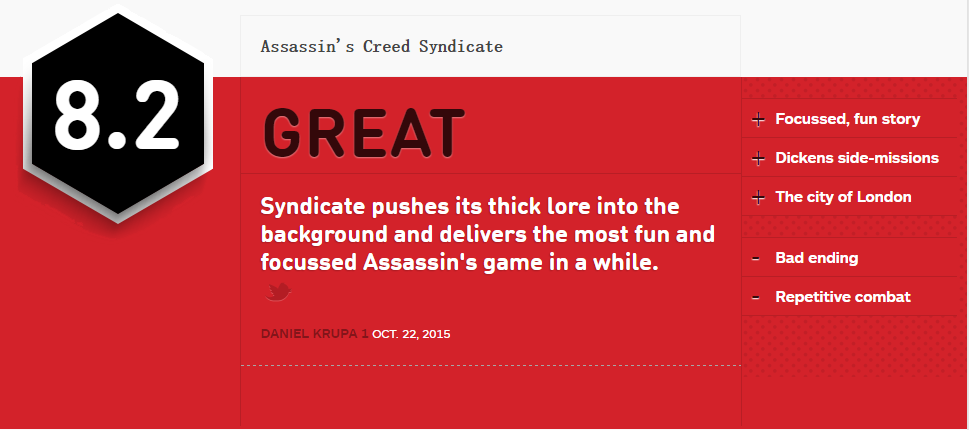
\includegraphics[width=30em]{IGN.png}\\
  \caption{IGN评分}\label{3-1}
\end{figure}
\paragraph{}
《刺客信条》一直强调画面和从前代传承下来的游戏机制,但是做的再好,没有突破,也难免会让玩家审美疲劳。育碧也许是时候做出突破了,否则下一代刺客信条也许就只能消费玩家的信仰了。


\end{document}
